\section{The Hunt for Dark Matter}

The astronomical evidence for \acrfull{dm}, from galaxy rotation curves to the \acrfull{cmb}, establishes the need for terrestrial detection experiments. This chapter traces how decades of cosmological observations have shaped our understanding of \acrshort{dm} properties, directly informing the detection strategies employed in XENONnT where precise signal classification becomes crucial for identifying potential \acrshort{dm} interactions.

\subsection{The Cosmic Microwave Background}

The \acrshort{cmb} is the leftover radiation released during recombination \cite{Wilson_CMB_obs}. It encodes information that helps us probe and test different cosmological models. To explain these observations we see in the \gls{cmb}, we need a form of matter that does not interact with light. We call this \acrshort{dm}. The CMB also encodes the total matter-energy content of the universe and the fractional densities of each of these components, $\Omega_m =0.05$ for baryonic matter and $\Omega_{DM} =0.27$ for \acrshort{dm} \cite{Planck2020, Dodelson2003}. This shows that \acrshort{dm} is at least 5 times as abundant as baryonic matter.

\begin{figure}[ht!]
    \centering
    \includegraphics[width=0.5\linewidth]{figs/intro_figs/CMB_comparison.png}
    \caption{CMB temperature fluctuation simulation at 1$\degree$ angular observation. This simulation was generated with CMB simulator \cite{North2023} and shows what the \gls{cmb} would look like if we set dark matter to zero. Top right corner of the image shows the observed CMB fluctuations.}
    \label{fig:CMB_comparison}
\end{figure}

Before recombination, the baryon-photon plasma that permeated the universe underwent acoustic oscillations resulting mainly from the competing forces of gravitational potential and radiation pressure \cite{Kolb1990}. Since \acrshort{dm} is collisionless and does not interact with light, it served to strengthen some of these gravitational wells without oscillating due to the radiation pressure. 

During recombination (z=1,100), the average temperature of the universe dropped below 3,000K \cite{Weinberg1972}. At these temperatures, protons and electrons could combine to form neutral hydrogen atoms. This meant that the mean free path of photons became larger than the Hubble Radius, creating the surface of last scattering observed as the \gls{cmb}. After cooling, modern calculations yield an average CMB temperature at 2.725\,$K$ \cite{Fixsen_2009} with anisotropies at the level of $\pm 400\,\micro K$ \cite{Planck:2013lks}. These fluctuations, though small, reveal the composition of the early universe.

\begin{figure}[ht!]
    \centering
    \includegraphics[width=0.9\linewidth]{figs/intro_figs/cmb_power_spectrum.jpg}
    \caption{Power spectrum of the temperature fluctuations of the \gls{cmb} as a function of angular size and multipole moment $l$. The first three peaks are used to understand the relative abundance of baryonic and DM in the Universe.}
    \label{fig:CMB_power_spectrum}
\end{figure}

By analyzing the fluctuations in the \gls{cmb} and computing its power spectrum (Fig. \ref{fig:CMB_power_spectrum}) we can determine the matter-energy content distribution of the universe based on the observed peaks \cite{Sunyaev1970, Peebles1970}. The relative heights of the first three peaks constrain the density of baryons and \acrshort{dm} independently. This provides model-independent evidence for non-baryonic \acrshort{dm}.

\begin{comment}

%Galaxy rotation curves and the Bullet Cluster provided some of the early hints for the existence of DM. However, the most compelling evidence for DM comes from the cosmic microwave background (CMB). By analyzing the baryonic acoustic oscillations resulting from the \gls{cmb}, we can test cosmological theories with unprecedented precision. The anisotropies in temperature fluctuations found here are used to deduce the state of the early universe and what components had to be present to result in the observations we see today.

To understand the most compelling evidence for dark matter, the \acrfull{cmb}, we first need to understand the Big Bang model. In 1924, Alexander Friedmann found solutions to Einstein’s equations of general relativity that did not require the universe to be static. For all solutions, if we trace the expansion backward in time, the universe converges to a singular state of extremely high density and temperature \cite{Friedmann1924, Friedmann1999},  the Big Bang.
In 1929, Edwin Hubble provided the first clear observational evidence for the expansion of the universe. By measuring the redshifts of galaxies, he showed that their recession velocity increased linearly with distance \cite{hubble_nebula_dist}. This relationship, now known as Hubble’s law, implies that the universe is expanding from an initial dense state. Such behavior was consistent with the expanding-universe solutions of Friedmann’s equations, giving credibility and laying the foundation for the Big Bang model.

% 10 MeV -> approx max binding energy per nucleon translates to roughtly 10^11 K
% 13eV -> 10^5 K binding energy of electron to a hydrogen atom
% CMB released at 3*10^4 K

In the first few hundred thousand years after the Big Bang, the universe was still extremely hot and dense, with an average temperature above 3000$\degree K$ and an average density at least 10 orders of magnitude higher than it is today \cite{Weinberg1972}. In this state, the constant collision of high-energy particles can produce any particle that is kinematically available in these conditions, including exotic particles like DM. Here, atoms could not yet form because the high energies kept electrons and protons from binding, and photons continuously scattered off these free particles. The main competing forces were gravity, pulling matter together, and photon pressure, pushing it apart. In addition to radiation and baryonic matter, a third component, dark matter, contributed significantly. Unlike baryons, dark matter was never coupled with radiation due to its lack of an electric charge; as such, it did not scatter with photons. Instead, it only contributed to the gravitational potential, deepening potential wells and allowing density fluctuations to grow \cite{Kolb1990}. 


The competition between photon pressure, driving matter outward, and gravity, pulling it inward, generated oscillations in the baryon–photon plasma. When the universe cooled enough for atoms to form, photons decoupled from matter in a process called recombination. The photons released then are observed today as the \gls{cmb} \cite{Wilson_CMB_obs} Fig. \ref{fig:CMB_plank_2013}. These oscillations left a distinctive imprint in the \gls{cmb}, seen today as temperature fluctuations which reveal the universe’s early composition.

\begin{figure}[ht!]
    \centering
    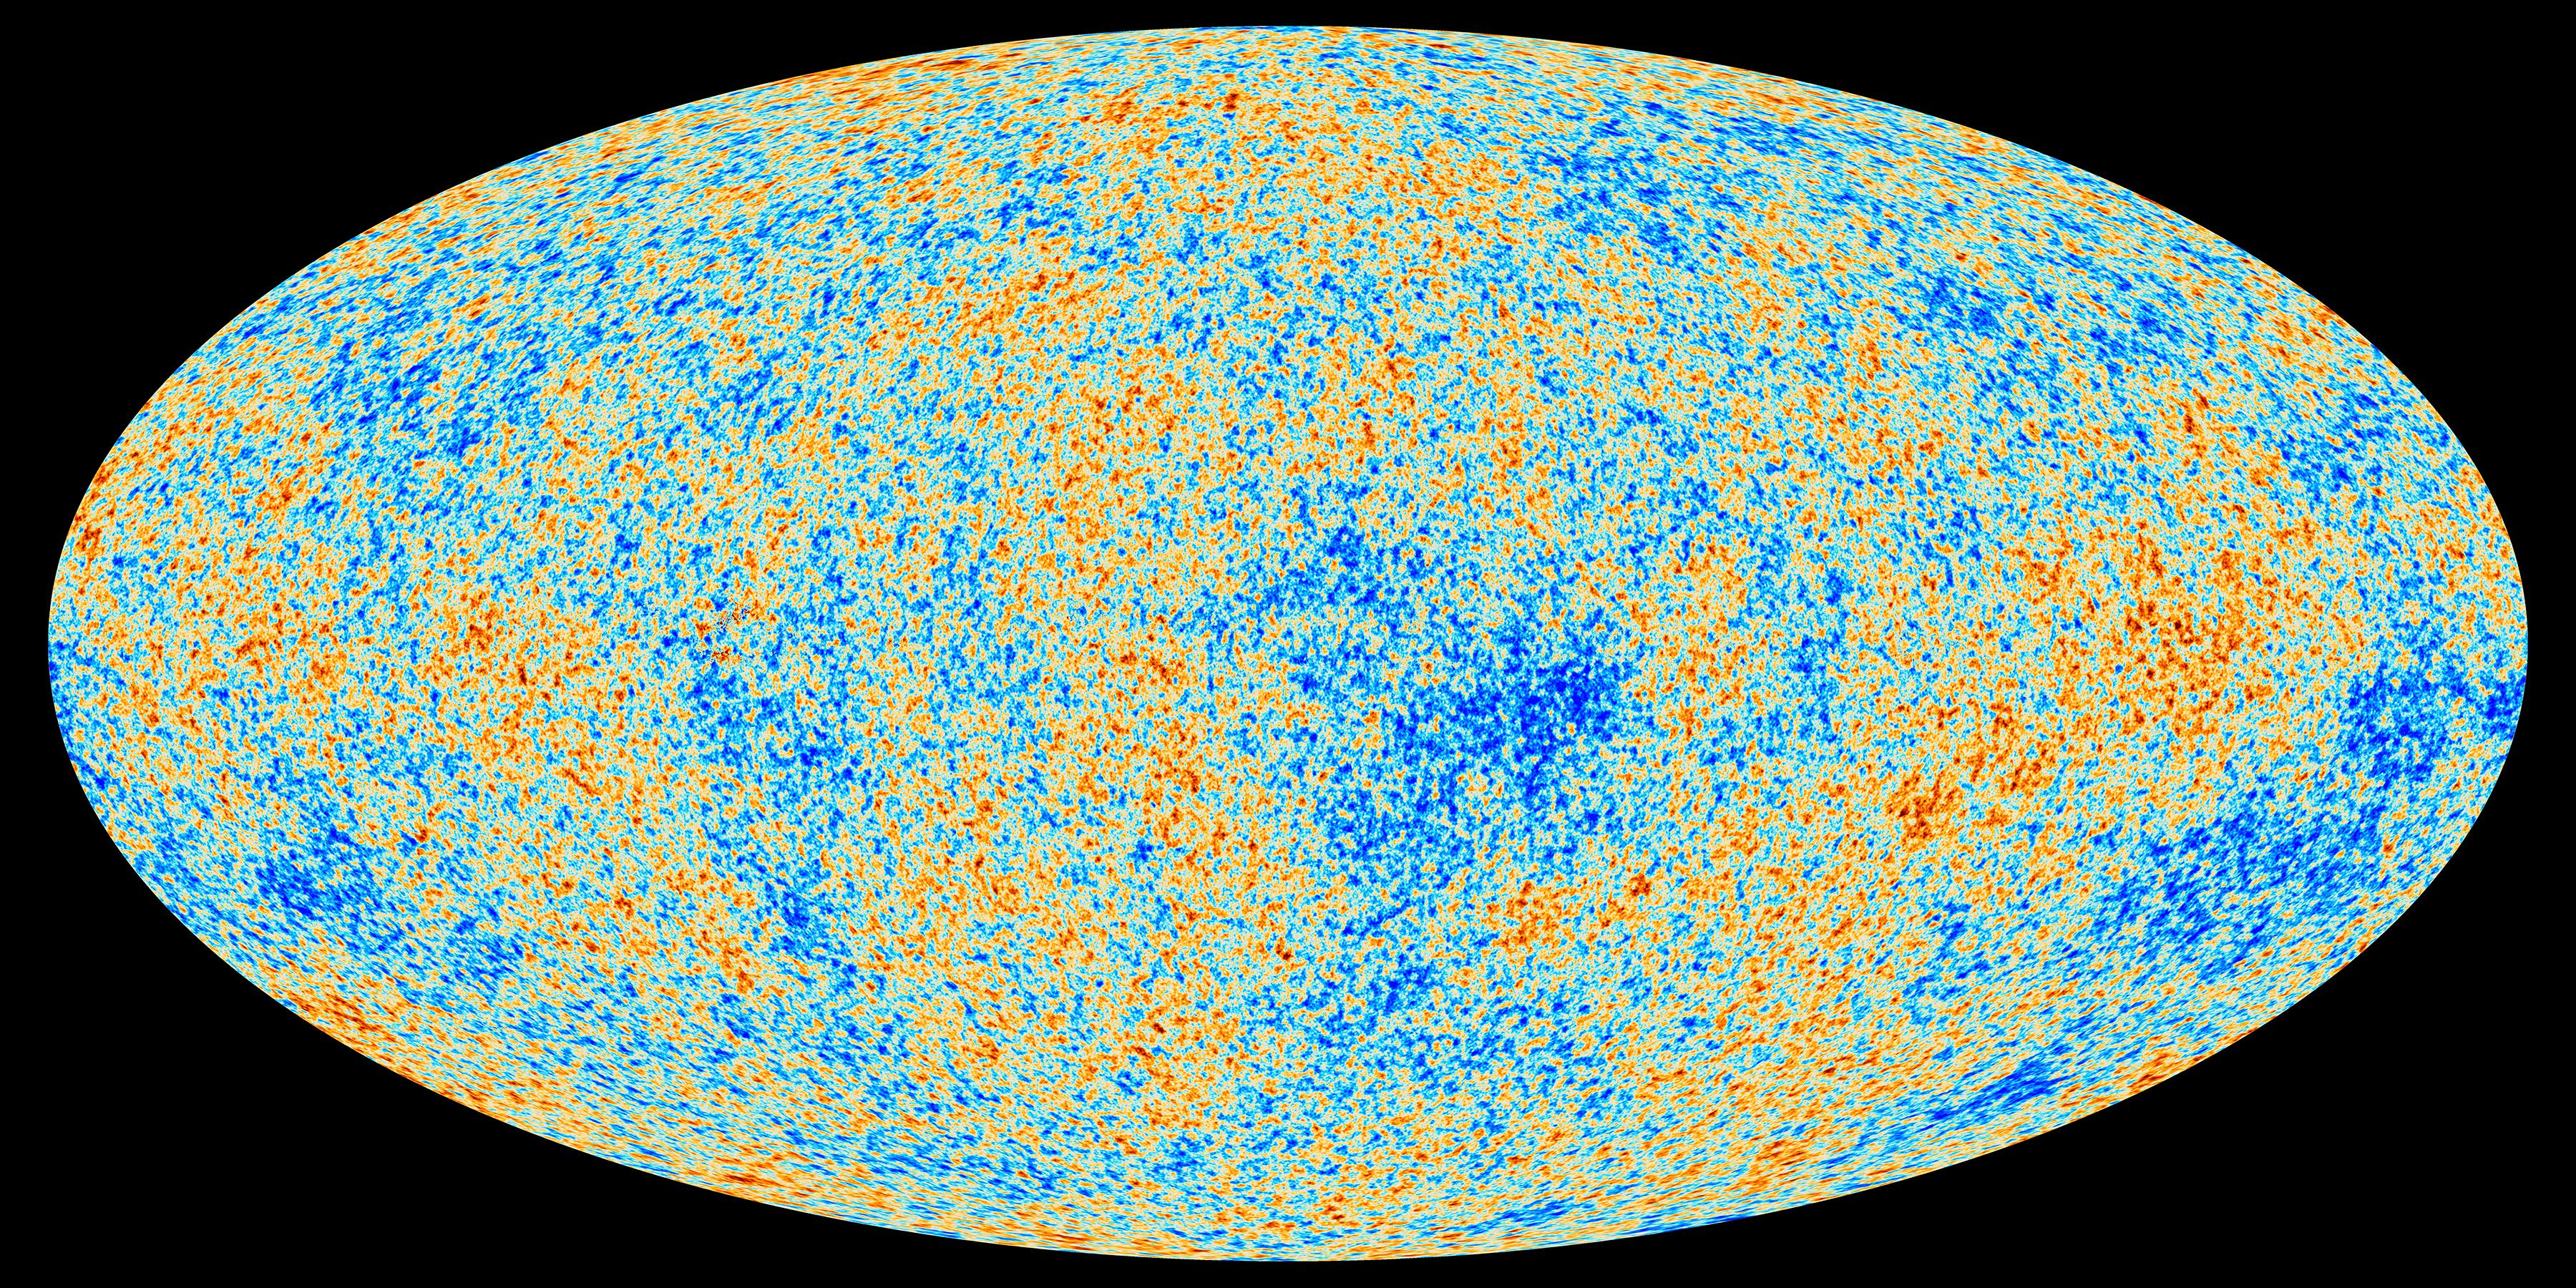
\includegraphics[width=0.9\linewidth]{figs/intro_figs/CMB_plank.png}
    \caption{Map showing the temperature fluctuations of the \gls{cmb} after all corrections are applied. The blue shows temperatures below the mean and the red shows temperatures above the mean. Image credit \cite{Planck:2013lks}}
    \label{fig:CMB_plank_2013}
\end{figure}

The Big Bang model predicts that relic radiation from the hot, dense early universe should still be observable today as a nearly uniform background. This prediction was confirmed in 1965, when Penzias and Wilson detected an unexpected, nearly isotropic background signal corresponding to a blackbody temperature of about 3.5\,$\degree K$ \cite{Wilson_CMB_obs}. More modern calculations have placed the average CMB temperature at 2.725\,$\degree K$ \cite{Fixsen_2009} with anisotropies at the level of $\pm 400\,\micro K$ \cite{Planck:2013lks}. These fluctuations, though small, provide one of our most powerful windows into the universe’s composition and early structure.

After applying necessary corrections to the \gls{cmb}, such as removing foreground emissions from the Milky Way, accounting for seasonal variations due to Earth’s orbital motion, and subtracting the Doppler, induced dipole anisotropy, we obtain the cleaned CMB map shown in Fig. \ref{fig:CMB_plank_2013}. Once these effects are removed, the remaining temperature fluctuations, though small, represent primordial anisotropies. These anisotropies provide detailed insight into the structure of the early universe and its physical composition. In particular, their characteristic scales encode the baryon–photon oscillations of the pre-recombination plasma.



The discovery of the \gls{cmb} provided an invaluable dataset, offering a glimpse into the early structure of the universe. Regions with higher matter density exhibited stronger oscillations, with the fundamental mode completing fewer than two full cycles before recombination. These oscillations imprinted themselves as peaks in the \gls{cmb} power spectrum, shown in Fig. \ref{fig:CMB_power_spectrum}. Each peak corresponds to a harmonic of the baryon–photon oscillations: odd peaks indicate compressions, while even peaks represent rarefactions. By analyzing the relative heights of these peaks, we can infer the amounts and types of matter and energy in the universe.



The peaks in this plot represent the strength (variance) of temperature fluctuations at different angular scales. Maximum variance occurs when the oscillations of the baryon–photon plasma are at either maximum compression (hotter regions) or maximum rarefaction (cooler regions). Odd-numbered peaks correspond to compressions, while even peaks correspond to rarefactions. The relative heights of the first and second peaks provide a measure of the baryon density: because baryons have inertia, the even peaks are suppressed compared to the odd ones. Dark matter, by contrast, does not couple to photons; it deepens gravitational potential wells without being affected by radiation pressure. In a universe with only baryons and photons, higher-order oscillations would be strongly damped, and the third peak would be suppressed relative to the second. Instead, observations show that the third peak is comparable in size, providing one of the clearest signatures of dark matter’s presence and abundance.

\end{comment}

\subsection{Cosmological Scale Evidence for Dark Matter}

\acrshort{dm} further helps explain the large-scale structure of the universe today. Without it, baryonic matter would not have had enough time to cool down via radiation to form the galaxies and galaxy clusters we see today. N-body simulations show that the distribution of galaxies and galaxy clusters we see today, including the cosmic web, could only be possible with \acrshort{dm} \cite{Benson_2010}. Under this theory, the small \acrshort{dm} halos that formed before recombination are expanded by inflation and some merge together over time. This leads to the formation of larger halos and more complex structures, leading to the universe we observe today \cite{cui2024knowhalomassfunction}. Further observations and calculations following the \gls{cmb} fluctuations to the present and analyzing the corresponding large-scale structure give further credibility to this claim \cite{sanchez_2011, PhysRevD.71.103515, Percival_2007}.


\subsection{Dark Matter Production}

To have the \acrshort{dm} we see in the universe, \acrshort{dm} must have a production mechanism, some way in which the high-energy early universe could produce \acrshort{dm}. Following Feynman's rules, if \acrshort{dm} has a creation mechanism, then it must also have an annihilation mechanism as Feynman diagrams are invertible \cite{PhysRev.76.769, Srednicki2007}. Under these conditions, over time \acrshort{dm} must have reached a thermal equilibrium in which it was being created and destroyed in equal amounts. As the universe expands and cools we can no longer generate new \acrshort{dm} particles. Later still in the evolution of the universe, \acrshort{dm} becomes sparse enough that annihilation interactions also do not happen. We refer to this process as ``freezeout" \cite{PhysRevLett.39.165}. After freezeout, the comoving number density for \acrshort{dm} is fixed and we calculate it as:

\begin{equation}
    \Omega_{\chi}h^2 = \frac{3 \times10^{-27}\frac{\text{cm}^3}{s}}{\langle\sigma v\rangle}.
    \label{dm_density}
\end{equation}

Now, for \acrfull{wimp}, dimensional analysis gives us $\langle\sigma v\rangle \approx \alpha^2/m^2_{\chi}$. If we plug in a value of 100\,GeV, which is in the weak scale, this gives us $\langle\sigma v\rangle = 3\times10^{-26}cm^3/s$ \cite{Steigman_2012}. Remarkably, when we now compute Eq. \ref{dm_density}, this gives a value of 0.1, which matches the observations with a value of 0.12. This is known as the \gls{wimp} miracle. 

This furthermore gives us a good insight into how to detect \acrshort{dm}. If we want to detect \acrshort{dm} via scattering with baryonic matter, we want to maximize the amount of energy imparted by the \acrshort{dm} particle onto our baryonic matter. For this we want full elastic scattering, so we want to use a target mass that is approximately 100\,GeV \cite{V_Chepel_2013}. Xenon happens to fit this bill with its most abundant isotope having a mass of $\approx 123$\,GeV.



\subsection{Current Knowledge of Dark Matter}

With the observational evidence for \gls{dm} established, the next step is to ask: what could it be? To guide this search, it is useful to first outline the key properties of \gls{dm}. From the evidence discussed in previous sections, we can infer the following properties of \acrshort{dm}:

\begin{itemize}
    \item \textbf{\acrshort{dm} is effectively electromagnetically neutral.} This comes from the \gls{cmb} power spectrum, since if \acrshort{dm} were strongly coupled to photons, this would be reflected in the fluctuations of the \gls{cmb} \cite{McDermott_2011}. 
    \item \textbf{\acrshort{dm} is effectively non-self interacting.} Observations of the Bullet Cluster show that if \acrshort{dm} were strongly self-interacting, its distribution would diverge from that of galaxies. Instead, it follows the galaxies, which behave like a collisionless gas \cite{Buote_2002, Harvey:2015hha}. 

    \item \textbf{\acrshort{dm} cannot be `hot'.} It does not move at relativistic speeds, since this would contradict the observed structure formation of the universe.
    
    \item \textbf{\acrshort{dm} has a minimum mass scale, depending on whether it is fermionic or bosonic.} The lower limits for fermionic \acrshort{dm} can be derived using Pauli's exclusion principle combined with the cosmological observations of galaxies and galaxy clusters, resulting in a lower limit of 70\,eV \cite{PhysRevLett.42.407, Randall:2016bqw}. In order to not conflict with the observations of the \gls{cmb}, bosonic \acrshort{dm} has a lower limit of $10^{-22}$\,eV \cite{Schive_2016, Nadler_2019}.
    
    \item \textbf{\acrshort{dm} is stable.} With a life-time comparable to or greater than the age of the universe, since it plays a key role in late-time structure formation. Estimates on the half-life of \gls{dm} have given it a lower value of 160\,Gyr \cite{Audren_2014}. In particular, the galaxy clusters we observe are not compatible with a large DM decay.
    
\end{itemize}

These constraints are stringent: combined, they exclude all known Standard Model particles. Any charged particle is ruled out, eliminating all quarks, charged leptons, and the W bosons. Neutrinos are fermions and have an upper bound mass estimate of 0.45\,eV \cite{KATRIN:2021uub}, much lower than the fermionic \gls{dm} 70\,eV limit. Gluons and photons are excluded because they are massless. Finally, the stability requirement rules out the Higgs and Z boson. %Not only this but due to the results of recent dark matter experiments, most of the fundamental forces have been ruled out of the WIMP paradigm as possible modes of interaction between WIMPs and baryonic matter \cite{Escudero:2016gzx}.

Alternative theories, such as modified gravity, have been proposed. However, none can simultaneously explain galaxy rotation curves, the Bullet Cluster, and the detailed features of the \gls{cmb}, which together probe \acrshort{dm} on galactic, cluster, and cosmological scales. These independent lines of evidence strongly favor a new particle component beyond the Standard Model. Among the many proposed candidates, one of the most theoretically well-motivated is the \gls{wimp}.



\subsection{Dark Matter Candidates}


\Glspl{wimp} are considered “massive” particles because their expected mass range lies between 20\,GeV and 100\,TeV \cite{Leane:2018kjk}, significantly heavier than most Standard Model particles. Direct detection experiments have already excluded large regions of the parameter space for \glspl{wimp} interacting via the weak nuclear force or the Higgs mechanism \cite{Escudero_2016}. Furthermore, from these experiments we have also ruled out \gls{dm}-nucleon cross section until regions close to the neutrino fog, the current \gls{dm}-nucleon cross section limits can be seen in Fig. \ref{fig:DM-nucleon_cs}. Nevertheless, this does not rule out \glspl{wimp} entirely; there remains the possibility that their interactions are mediated by a yet undiscovered fundamental force beyond the Standard Model.

\begin{figure}
    \centering
    \includegraphics[width=0.8\linewidth]{figs/intro_figs/DM-nucleon_cross_section.png}
    \caption{\acrshort{dm}-nucleon cross section as a function of \acrshort{dm} mass. Here we see the current limits from a variety of experiments. LZ has placed the most stringent limits for masses between 10 and 1,000\,GeV \cite{ref1, ref2, ref3, ref4, ref5, ref6, ref7, ref8, ref9, ref10, ref11, ref12, ref13, ref14, ref15, ref16, ref17}. Figure was generated using the \acrshort{dm} limit plotter made by Tarek Saab, University of Florida and Enectali Figueroa, Northwestern University.}
    \label{fig:DM-nucleon_cs}
\end{figure}

% Add cication ot the models
% Talk about pros and cons of each model

Several other \acrshort{dm} candidates have been proposed. Axions \cite{PhysRevLett.40.223, axion_paper}, for example, are a theoretical particle proposed as a solution to the unexpected absence of \acrfull{cp}-violation derived from quantum chromo-dynamics \cite{cp_problem_sym}. Axions are a good candidate for \acrshort{dm} due to their strong theoretical background; they could also be produced in the early universe just like \glspl{wimp}. Furthermore, their production mechanism makes them likely to be ``cold" today \cite{Sikivie_2008} and naturally give the correct abundance for \acrshort{dm} without fine-tuning \cite{DiLuzio:2020wdo}.

Primordial black holes are also a compelling candidate for \acrshort{dm}. Unlike black holes formed from dead stars, these black holes would be produced in overdense regions in the early universe \cite{blackhole_early_uni, PhysRevD.50.7173}. These black holes can span 40 orders of magnitude in mass ranges so there is a lot of flexibility in the possible masses \cite{PhysRevD.94.083504, bh_mass_constraint_1975}. Furthermore, black holes would not be affected by the radiation pressure in the early universe, matching the characteristics we know of \acrshort{dm} from CMB observations.

While these candidates are also very promising as \acrshort{dm}, we will not expand on them any further in this text. The XENONnT experiment is optimized to probe Weakly Interacting Massive Particles (\glspl{wimp}), making them the primary focus of this thesis. Here we will explain the xenon experiment, both in terms of hardware and software. Then, we will discuss unsupervised neural networks and how they are used to improve the signal classification in the XENONnT experiment. Finally, we will take a brief look at XAMS, a small \acrfull{tpc} experiment used to test the \gls{tpc} technology and see the impact of unsupervised classification on this data.


\newpage